

For this task, artificial complex data was created to test two different antenna array layouts to obtain AOA coverage data: one with a circular and one with a spiral antenna distribution, each having 6 antennas. The array geometries can be seen in figures \ref{fig:t7-geo-circ} and \ref{fig:t7-geo-spir}.\\

Due to the low number of antennas, the main lobe in the antenna factor is relatively broad for both array types. The spiral array factor has a broader main lobe since the antennas along the spiral are spaced closer together. In any case, the vertical angle can be clearly seen from the array factor patterns (figures \ref{fig:t7-rad-circ} and \ref{fig:t7-rad-spir}) when steering the antennas with equal phases.\\

The result of the AOA calculations with the random data can be seen in figures \ref{fig:t7-aoa-circ} and \ref{fig:t7-aoa-spir}. As expected from the array factors, the spiral array shows a broader AOA coverage than the circular array type and both are pointing vertically. The grating lobes of the circular array show greater magnitude, so that aliasing might be greater. But in both array cases, the grating lobes lie almost on the edge of the horizon, which might result in negligible aliasing effects.

\begin{figure}
    \centering
    \begin{minipage}{0.48\textwidth}
        \centering
        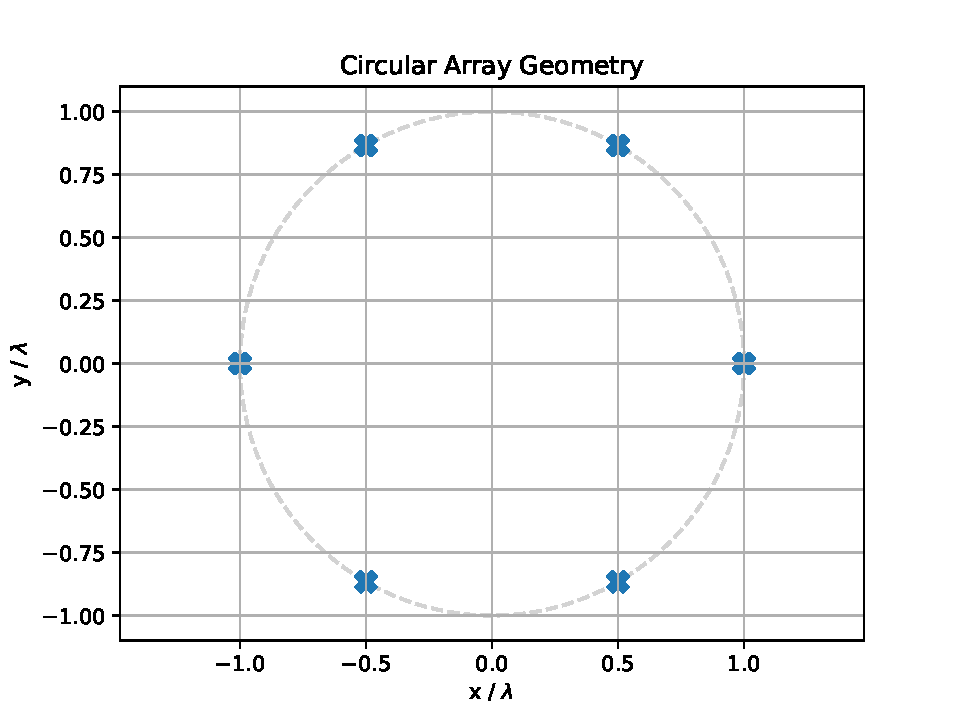
\includegraphics[width=1.0\textwidth]{graphics/t7/t7-geo-circ.pdf} % first figure itself
        \caption{Task 7: Array geometry of the circular array.}
        \label{fig:t7-geo-circ}
    \end{minipage}\hfill
    \begin{minipage}{0.48\textwidth}
        \centering
        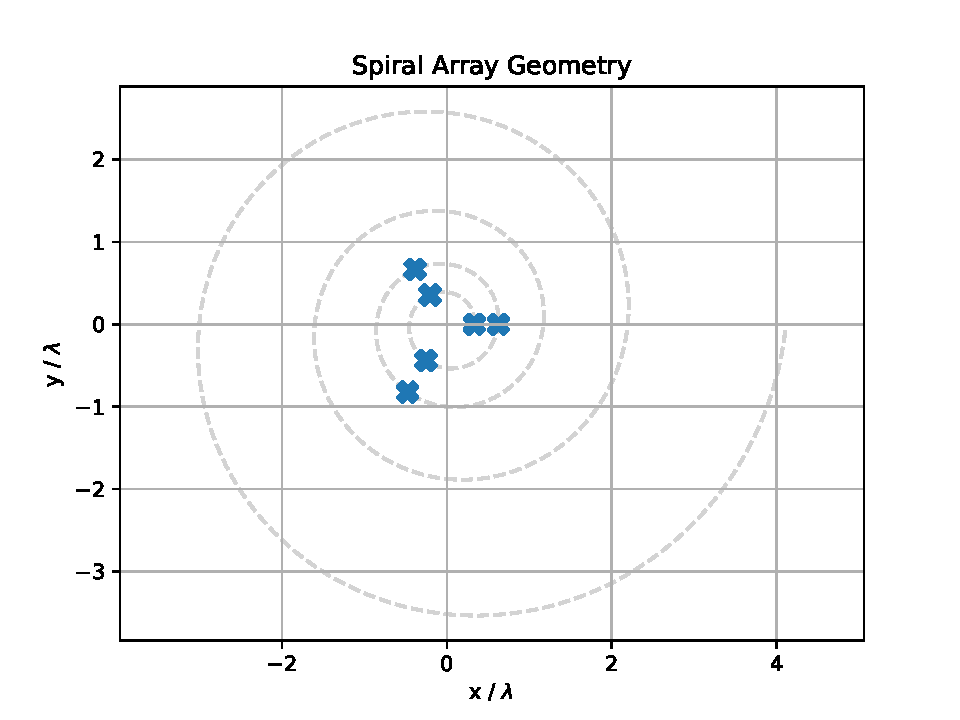
\includegraphics[width=1\textwidth]{graphics/t7/t7-geo-spir.pdf} % second figure itself
        \caption{Task 7: Array geometry of the spiral array.}
        \label{fig:t7-geo-spir}
    \end{minipage}
\end{figure}

\begin{figure}
    \centering
    \begin{minipage}{0.48\textwidth}
        \centering
        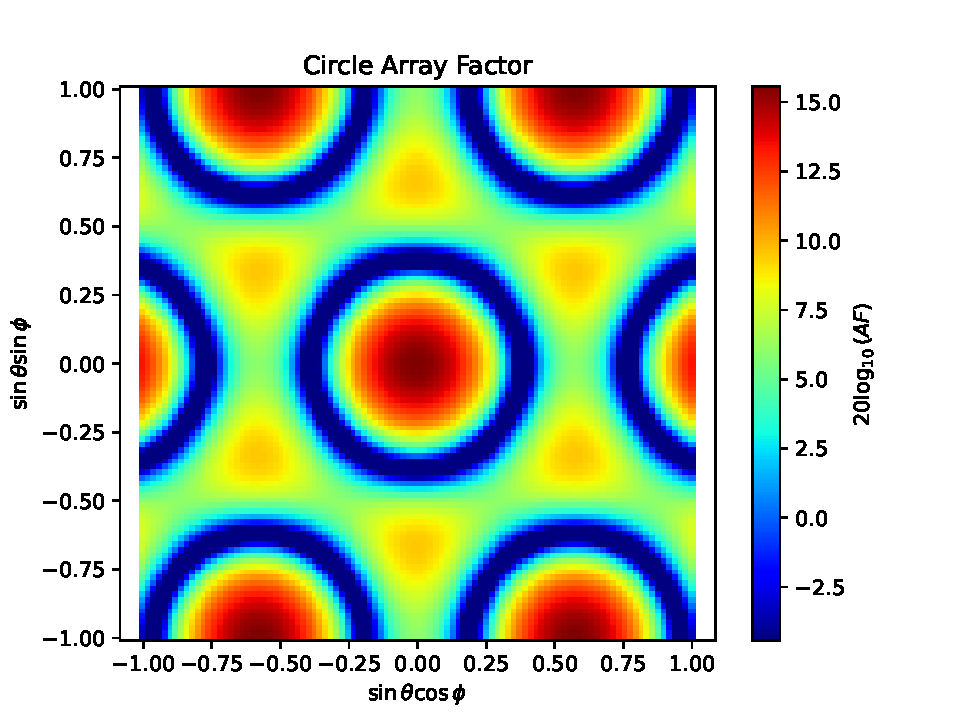
\includegraphics[width=1.0\textwidth]{graphics/t7/t7-rad-circ.pdf} % first figure itself
        \caption{Task 7: Array factor of circular array.}
        \label{fig:t7-rad-circ}
    \end{minipage}\hfill
    \begin{minipage}{0.48\textwidth}
        \centering
        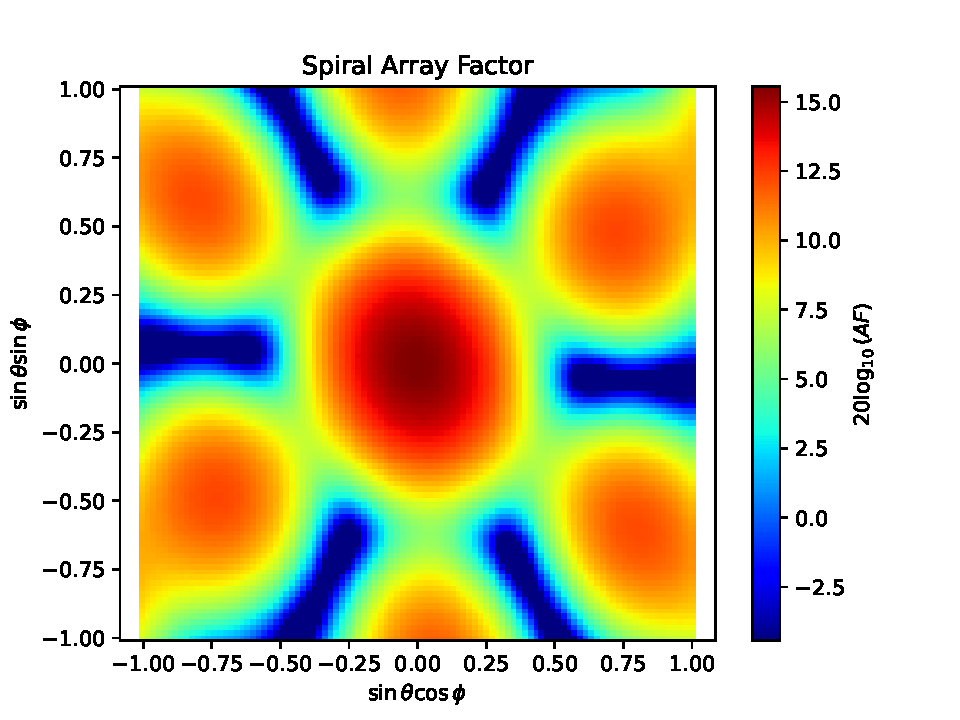
\includegraphics[width=1\textwidth]{graphics/t7/t7-rad-spir.pdf} % second figure itself
        \caption{Task 7: Array factor of spiral array.}
        \label{fig:t7-rad-spir}
    \end{minipage}
\end{figure}

\begin{figure}
    \centering
    \begin{minipage}{0.48\textwidth}
        \centering
        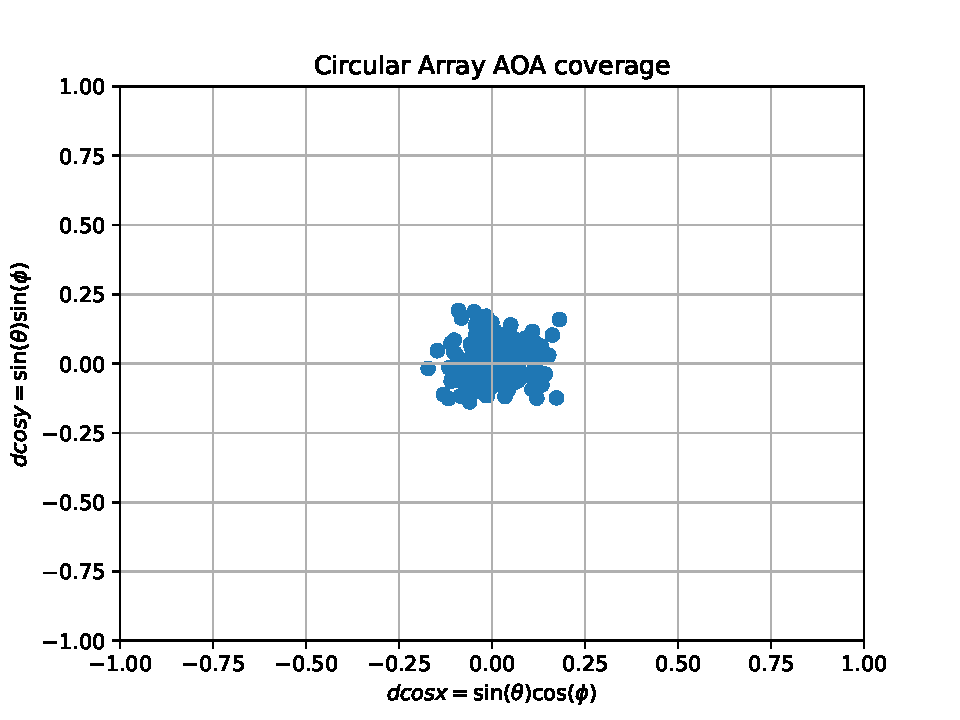
\includegraphics[width=1.0\textwidth]{graphics/t7/t7-aoa-circ.pdf} % first figure itself
        \caption{Task 7: AOA coverage of circular array.}
        \label{fig:t7-aoa-circ}
    \end{minipage}\hfill
    \begin{minipage}{0.48\textwidth}
        \centering
        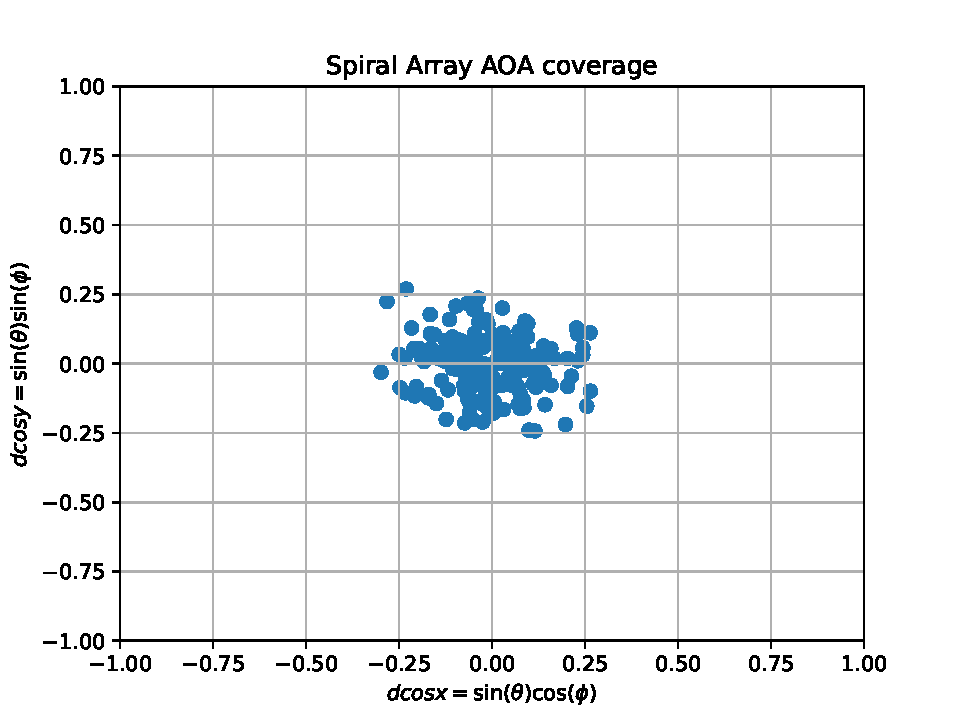
\includegraphics[width=1\textwidth]{graphics/t7/t7-aoa-spir.pdf} % second figure itself
        \caption{Task 7: AOA coverage of spiral array.}
        \label{fig:t7-aoa-spir}
    \end{minipage}
\end{figure}
